\documentclass[1p]{elsarticle_modified}
%\bibliographystyle{elsarticle-num}

%\usepackage[colorlinks]{hyperref}
%\usepackage{abbrmath_seonhwa} %\Abb, \Ascr, \Acal ,\Abf, \Afrak
\usepackage{amsfonts}
\usepackage{amssymb}
\usepackage{amsmath}
\usepackage{amsthm}
\usepackage{scalefnt}
\usepackage{amsbsy}
\usepackage{kotex}
\usepackage{caption}
\usepackage{subfig}
\usepackage{color}
\usepackage{graphicx}
\usepackage{xcolor} %% white, black, red, green, blue, cyan, magenta, yellow
\usepackage{float}
\usepackage{setspace}
\usepackage{hyperref}

\usepackage{tikz}
\usetikzlibrary{arrows}

\usepackage{multirow}
\usepackage{array} % fixed length table
\usepackage{hhline}

%%%%%%%%%%%%%%%%%%%%%
\makeatletter
\renewcommand*\env@matrix[1][\arraystretch]{%
	\edef\arraystretch{#1}%
	\hskip -\arraycolsep
	\let\@ifnextchar\new@ifnextchar
	\array{*\c@MaxMatrixCols c}}
\makeatother %https://tex.stackexchange.com/questions/14071/how-can-i-increase-the-line-spacing-in-a-matrix
%%%%%%%%%%%%%%%

\usepackage[normalem]{ulem}

\newcommand{\msout}[1]{\ifmmode\text{\sout{\ensuremath{#1}}}\else\sout{#1}\fi}
%SOURCE: \msout is \stkout macro in https://tex.stackexchange.com/questions/20609/strikeout-in-math-mode

\newcommand{\cancel}[1]{
	\ifmmode
	{\color{red}\msout{#1}}
	\else
	{\color{red}\sout{#1}}
	\fi
}

\newcommand{\add}[1]{
	{\color{blue}\uwave{#1}}
}

\newcommand{\replace}[2]{
	\ifmmode
	{\color{red}\msout{#1}}{\color{blue}\uwave{#2}}
	\else
	{\color{red}\sout{#1}}{\color{blue}\uwave{#2}}
	\fi
}

\newcommand{\Sol}{\mathcal{S}} %segment
\newcommand{\D}{D} %diagram
\newcommand{\A}{\mathcal{A}} %arc


%%%%%%%%%%%%%%%%%%%%%%%%%%%%%5 test

\def\sl{\operatorname{\textup{SL}}(2,\Cbb)}
\def\psl{\operatorname{\textup{PSL}}(2,\Cbb)}
\def\quan{\mkern 1mu \triangleright \mkern 1mu}

\theoremstyle{definition}
\newtheorem{thm}{Theorem}[section]
\newtheorem{prop}[thm]{Proposition}
\newtheorem{lem}[thm]{Lemma}
\newtheorem{ques}[thm]{Question}
\newtheorem{cor}[thm]{Corollary}
\newtheorem{defn}[thm]{Definition}
\newtheorem{exam}[thm]{Example}
\newtheorem{rmk}[thm]{Remark}
\newtheorem{alg}[thm]{Algorithm}

\newcommand{\I}{\sqrt{-1}}
\begin{document}

%\begin{frontmatter}
%
%\title{Boundary parabolic representations of knots up to 8 crossings}
%
%%% Group authors per affiliation:
%\author{Yunhi Cho} 
%\address{Department of Mathematics, University of Seoul, Seoul, Korea}
%\ead{yhcho@uos.ac.kr}
%
%
%\author{Seonhwa Kim} %\fnref{s_kim}}
%\address{Center for Geometry and Physics, Institute for Basic Science, Pohang, 37673, Korea}
%\ead{ryeona17@ibs.re.kr}
%
%\author{Hyuk Kim}
%\address{Department of Mathematical Sciences, Seoul National University, Seoul 08826, Korea}
%\ead{hyukkim@snu.ac.kr}
%
%\author{Seokbeom Yoon}
%\address{Department of Mathematical Sciences, Seoul National University, Seoul, 08826,  Korea}
%\ead{sbyoon15@snu.ac.kr}
%
%\begin{abstract}
%We find all boundary parabolic representation of knots up to 8 crossings.
%
%\end{abstract}
%\begin{keyword}
%    \MSC[2010] 57M25 
%\end{keyword}
%
%\end{frontmatter}

%\linenumbers
%\tableofcontents
%
\newcommand\colored[1]{\textcolor{white}{\rule[-0.35ex]{0.8em}{1.4ex}}\kern-0.8em\color{red} #1}%
%\newcommand\colored[1]{\textcolor{white}{ #1}\kern-2.17ex	\textcolor{white}{ #1}\kern-1.81ex	\textcolor{white}{ #1}\kern-2.15ex\color{red}#1	}

{\Large $\underline{12n_{0813}~(K12n_{0813})}$}

\setlength{\tabcolsep}{10pt}
\renewcommand{\arraystretch}{1.6}
\vspace{1cm}\begin{tabular}{m{100pt}>{\centering\arraybackslash}m{274pt}}
\multirow{5}{120pt}{
	\centering
	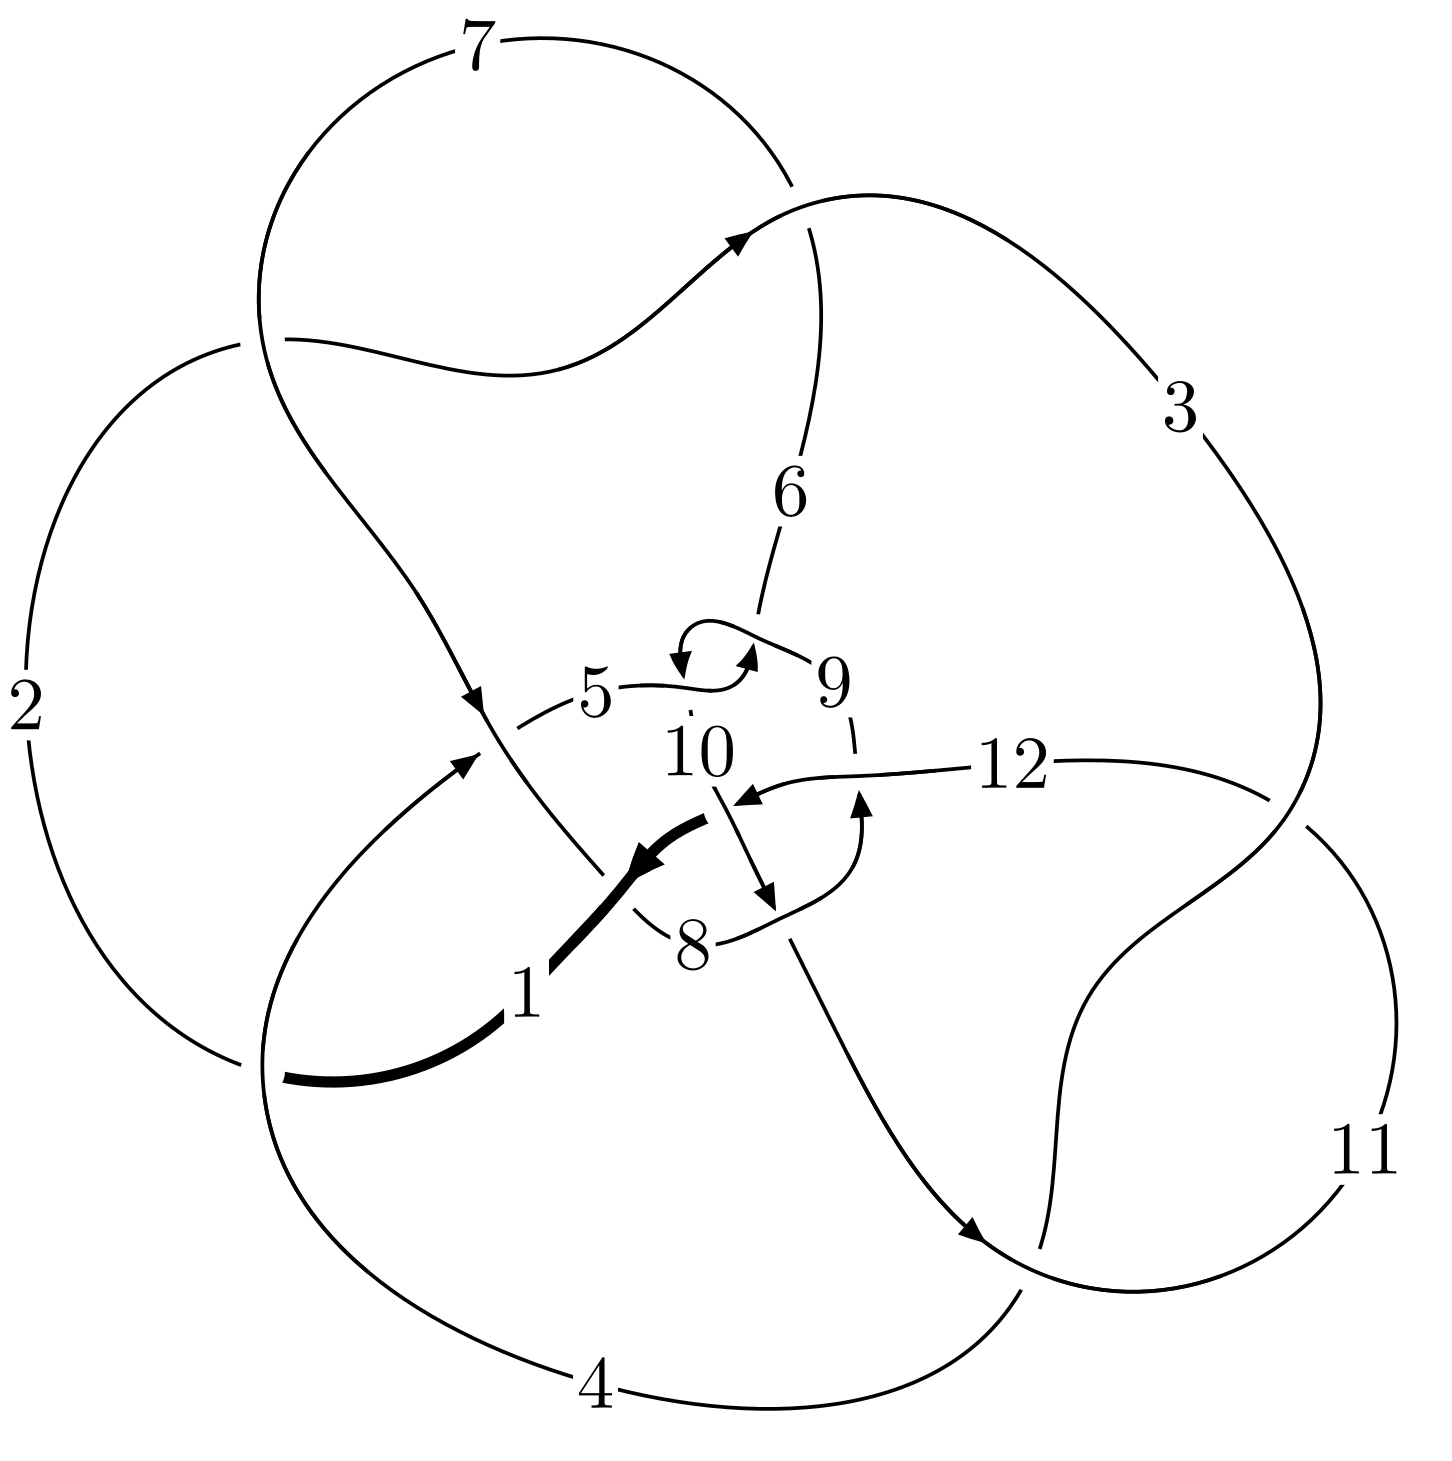
\includegraphics[width=112pt]{../../../GIT/diagram.site/Diagrams/png/2902_12n_0813.png}\\
\ \ \ A knot diagram\footnotemark}&
\allowdisplaybreaks
\textbf{Linearized knot diagam} \\
\cline{2-2}
 &
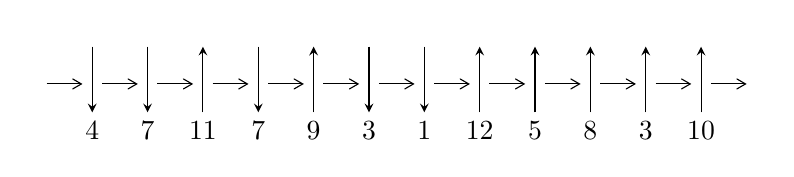
\begin{tikzpicture}[x=20pt, y=17pt]
	% nodes
	\node (C0) at (0, 0) {};
	\node (C1) at (1, 0) {};
	\node (C1U) at (1, +1) {};
	\node (C1D) at (1, -1) {4};

	\node (C2) at (2, 0) {};
	\node (C2U) at (2, +1) {};
	\node (C2D) at (2, -1) {7};

	\node (C3) at (3, 0) {};
	\node (C3U) at (3, +1) {};
	\node (C3D) at (3, -1) {11};

	\node (C4) at (4, 0) {};
	\node (C4U) at (4, +1) {};
	\node (C4D) at (4, -1) {7};

	\node (C5) at (5, 0) {};
	\node (C5U) at (5, +1) {};
	\node (C5D) at (5, -1) {9};

	\node (C6) at (6, 0) {};
	\node (C6U) at (6, +1) {};
	\node (C6D) at (6, -1) {3};

	\node (C7) at (7, 0) {};
	\node (C7U) at (7, +1) {};
	\node (C7D) at (7, -1) {1};

	\node (C8) at (8, 0) {};
	\node (C8U) at (8, +1) {};
	\node (C8D) at (8, -1) {12};

	\node (C9) at (9, 0) {};
	\node (C9U) at (9, +1) {};
	\node (C9D) at (9, -1) {5};

	\node (C10) at (10, 0) {};
	\node (C10U) at (10, +1) {};
	\node (C10D) at (10, -1) {8};

	\node (C11) at (11, 0) {};
	\node (C11U) at (11, +1) {};
	\node (C11D) at (11, -1) {3};

	\node (C12) at (12, 0) {};
	\node (C12U) at (12, +1) {};
	\node (C12D) at (12, -1) {10};
	\node (C13) at (13, 0) {};

	% arrows
	\draw[->,>={angle 60}]
	(C0) edge (C1) (C1) edge (C2) (C2) edge (C3) (C3) edge (C4) (C4) edge (C5) (C5) edge (C6) (C6) edge (C7) (C7) edge (C8) (C8) edge (C9) (C9) edge (C10) (C10) edge (C11) (C11) edge (C12) (C12) edge (C13) ;	\draw[->,>=stealth]
	(C1U) edge (C1D) (C2U) edge (C2D) (C3D) edge (C3U) (C4U) edge (C4D) (C5D) edge (C5U) (C6U) edge (C6D) (C7U) edge (C7D) (C8D) edge (C8U) (C9D) edge (C9U) (C10D) edge (C10U) (C11D) edge (C11U) (C12D) edge (C12U) ;
	\end{tikzpicture} \\
\hhline{~~} \\& 
\textbf{Solving Sequence} \\ \cline{2-2} 
 &
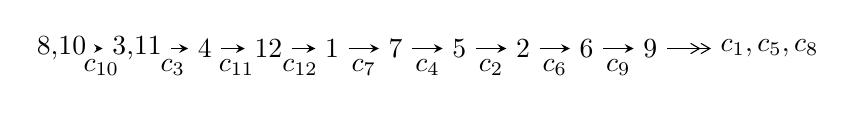
\begin{tikzpicture}[x=23pt, y=7pt]
	% node
	\node (A0) at (-1/8, 0) {8,10};
	\node (A1) at (17/16, 0) {3,11};
	\node (A2) at (17/8, 0) {4};
	\node (A3) at (25/8, 0) {12};
	\node (A4) at (33/8, 0) {1};
	\node (A5) at (41/8, 0) {7};
	\node (A6) at (49/8, 0) {5};
	\node (A7) at (57/8, 0) {2};
	\node (A8) at (65/8, 0) {6};
	\node (A9) at (73/8, 0) {9};
	\node (C1) at (1/2, -1) {$c_{10}$};
	\node (C2) at (13/8, -1) {$c_{3}$};
	\node (C3) at (21/8, -1) {$c_{11}$};
	\node (C4) at (29/8, -1) {$c_{12}$};
	\node (C5) at (37/8, -1) {$c_{7}$};
	\node (C6) at (45/8, -1) {$c_{4}$};
	\node (C7) at (53/8, -1) {$c_{2}$};
	\node (C8) at (61/8, -1) {$c_{6}$};
	\node (C9) at (69/8, -1) {$c_{9}$};
	\node (A10) at (11, 0) {$c_{1},c_{5},c_{8}$};

	% edge
	\draw[->,>=stealth]	
	(A0) edge (A1) (A1) edge (A2) (A2) edge (A3) (A3) edge (A4) (A4) edge (A5) (A5) edge (A6) (A6) edge (A7) (A7) edge (A8) (A8) edge (A9) ;
	\draw[->>,>={angle 60}]	
	(A9) edge (A10);
\end{tikzpicture} \\ 

\end{tabular} \\

\footnotetext{
The image of knot diagram is generated by the software ``\textbf{Draw programme}" developed by Andrew Bartholomew(\url{http://www.layer8.co.uk/maths/draw/index.htm\#Running-draw}), where we modified some parts for our purpose(\url{https://github.com/CATsTAILs/LinksPainter}).
}\phantom \\ \newline 
\centering \textbf{Ideals for irreducible components\footnotemark of $X_{\text{par}}$} 
 
\begin{align*}
I^u_{1}&=\langle 
-771111978722 u^{20}+1238251991594 u^{19}+\cdots+10836897427858 b+3727293790301,\\
\phantom{I^u_{1}}&\phantom{= \langle  }-4119811015012 u^{20}+1626728296443 u^{19}+\cdots+5418448713929 a+9392161389977,\\
\phantom{I^u_{1}}&\phantom{= \langle  }u^{21}-8 u^{18}+\cdots-4 u-1\rangle \\
I^u_{2}&=\langle 
2.42041\times10^{171} u^{57}+5.72134\times10^{171} u^{56}+\cdots+5.04153\times10^{173} b+9.75536\times10^{173},\\
\phantom{I^u_{2}}&\phantom{= \langle  }8.38866\times10^{171} u^{57}+3.51276\times10^{172} u^{56}+\cdots+2.52076\times10^{173} a+1.91905\times10^{174},\\
\phantom{I^u_{2}}&\phantom{= \langle  }u^{58}+4 u^{57}+\cdots+872 u+128\rangle \\
I^u_{3}&=\langle 
-5 u^9+5 u^8+12 u^7+18 u^6-41 u^5-21 u^4+7 u^3+79 u^2+17 b+3 u-28,\\
\phantom{I^u_{3}}&\phantom{= \langle  }-26 u^9-59 u^8-26 u^7+131 u^6+137 u^5-116 u^4-375 u^3-208 u^2+17 a+87 u+123,\\
\phantom{I^u_{3}}&\phantom{= \langle  }u^{10}+u^9- u^8-5 u^7+u^6+7 u^5+7 u^4-5 u^3-5 u^2+u+1\rangle \\
I^u_{4}&=\langle 
2.30529\times10^{30} u^{27}-1.47328\times10^{31} u^{26}+\cdots+2.21437\times10^{30} b+1.35121\times10^{30},\\
\phantom{I^u_{4}}&\phantom{= \langle  }6.64906\times10^{30} u^{27}-5.31889\times10^{31} u^{26}+\cdots+8.85748\times10^{30} a-3.64020\times10^{31},\;u^{28}-7 u^{27}+\cdots-6 u+1\rangle \\
I^u_{5}&=\langle 
b+1,\;a-1,\;u-1\rangle \\
\\
\end{align*}
\raggedright * 5 irreducible components of $\dim_{\mathbb{C}}=0$, with total 118 representations.\\
\footnotetext{All coefficients of polynomials are rational numbers. But the coefficients are sometimes approximated in decimal forms when there is not enough margin.}
\newpage
\renewcommand{\arraystretch}{1}
\centering \section*{I. $I^u_{1}= \langle -7.71\times10^{11} u^{20}+1.24\times10^{12} u^{19}+\cdots+1.08\times10^{13} b+3.73\times10^{12},\;-4.12\times10^{12} u^{20}+1.63\times10^{12} u^{19}+\cdots+5.42\times10^{12} a+9.39\times10^{12},\;u^{21}-8 u^{18}+\cdots-4 u-1 \rangle$}
\flushleft \textbf{(i) Arc colorings}\\
\begin{tabular}{m{7pt} m{180pt} m{7pt} m{180pt} }
\flushright $a_{8}=$&$\begin{pmatrix}0\\u\end{pmatrix}$ \\
\flushright $a_{10}=$&$\begin{pmatrix}1\\0\end{pmatrix}$ \\
\flushright $a_{3}=$&$\begin{pmatrix}0.760330 u^{20}-0.300220 u^{19}+\cdots-8.07239 u-1.73337\\0.0711562 u^{20}-0.114263 u^{19}+\cdots-0.839947 u-0.343945\end{pmatrix}$ \\
\flushright $a_{11}=$&$\begin{pmatrix}1\\- u^2\end{pmatrix}$ \\
\flushright $a_{4}=$&$\begin{pmatrix}0.942629 u^{20}-0.355006 u^{19}+\cdots-9.35289 u-2.37753\\0.0479865 u^{20}-0.0935026 u^{19}+\cdots-0.803102 u-0.289159\end{pmatrix}$ \\
\flushright $a_{12}=$&$\begin{pmatrix}-0.219243 u^{20}+0.0523993 u^{19}+\cdots-3.48114 u+2.80752\\- u\end{pmatrix}$ \\
\flushright $a_{1}=$&$\begin{pmatrix}-0.219243 u^{20}+0.0523993 u^{19}+\cdots-4.48114 u+2.80752\\- u\end{pmatrix}$ \\
\flushright $a_{7}=$&$\begin{pmatrix}-0.446182 u^{20}+0.175167 u^{19}+\cdots+6.28299 u-0.878517\\-0.0893615 u^{20}-0.0192813 u^{19}+\cdots+1.00965 u-0.0523993\end{pmatrix}$ \\
\flushright $a_{5}=$&$\begin{pmatrix}1.74610 u^{20}-0.337342 u^{19}+\cdots-10.8540 u-4.81375\\0.182299 u^{20}-0.0547859 u^{19}+\cdots-1.28050 u-0.644165\end{pmatrix}$ \\
\flushright $a_{2}=$&$\begin{pmatrix}0.0498962 u^{20}-0.0689951 u^{19}+\cdots-3.44956 u+0.288895\\-0.0745060 u^{20}-0.133557 u^{19}+\cdots-0.359376 u-0.0997824\end{pmatrix}$ \\
\flushright $a_{6}=$&$\begin{pmatrix}-1.19456 u^{20}+0.321015 u^{19}+\cdots+9.77795 u+2.14931\\-0.154049 u^{20}+0.0478163 u^{19}+\cdots+0.918068 u+0.233126\end{pmatrix}$ \\
\flushright $a_{9}=$&$\begin{pmatrix}-0.267459 u^{20}+0.213730 u^{19}+\cdots+6.26370 u-0.773718\\-0.0893615 u^{20}-0.0192813 u^{19}+\cdots+1.00965 u-0.0523993\end{pmatrix}$\\&\end{tabular}
\flushleft \textbf{(ii) Obstruction class $= -1$}\\~\\
\flushleft \textbf{(iii) Cusp Shapes $= \frac{11409897026945}{5418448713929} u^{20}+\frac{2927023670684}{5418448713929} u^{19}+\cdots-\frac{19517453412181}{5418448713929} u-\frac{26799066510012}{5418448713929}$}\\~\\
\newpage\renewcommand{\arraystretch}{1}
\flushleft \textbf{(iv) u-Polynomials at the component}\newline \\
\begin{tabular}{m{50pt}|m{274pt}}
Crossings & \hspace{64pt}u-Polynomials at each crossing \\
\hline $$\begin{aligned}c_{1},c_{4}\end{aligned}$$&$\begin{aligned}
&u^{21}- u^{20}+\cdots+12 u-1
\end{aligned}$\\
\hline $$\begin{aligned}c_{2},c_{6}\end{aligned}$$&$\begin{aligned}
&u^{21}+16 u^{20}+\cdots-1136 u-272
\end{aligned}$\\
\hline $$\begin{aligned}c_{3},c_{5},c_{9}\\c_{11}\end{aligned}$$&$\begin{aligned}
&u^{21}- u^{20}+\cdots+8 u-2
\end{aligned}$\\
\hline $$\begin{aligned}c_{7}\end{aligned}$$&$\begin{aligned}
&u^{21}-13 u^{20}+\cdots+640 u-64
\end{aligned}$\\
\hline $$\begin{aligned}c_{8}\end{aligned}$$&$\begin{aligned}
&u^{21}-13 u^{20}+\cdots+936 u-128
\end{aligned}$\\
\hline $$\begin{aligned}c_{10},c_{12}\end{aligned}$$&$\begin{aligned}
&u^{21}-8 u^{18}+\cdots-4 u-1
\end{aligned}$\\
\hline
\end{tabular}\\~\\
\newpage\renewcommand{\arraystretch}{1}
\flushleft \textbf{(v) Riley Polynomials at the component}\newline \\
\begin{tabular}{m{50pt}|m{274pt}}
Crossings & \hspace{64pt}Riley Polynomials at each crossing \\
\hline $$\begin{aligned}c_{1},c_{4}\end{aligned}$$&$\begin{aligned}
&y^{21}-29 y^{20}+\cdots+120 y-1
\end{aligned}$\\
\hline $$\begin{aligned}c_{2},c_{6}\end{aligned}$$&$\begin{aligned}
&y^{21}-20 y^{20}+\cdots+874880 y-73984
\end{aligned}$\\
\hline $$\begin{aligned}c_{3},c_{5},c_{9}\\c_{11}\end{aligned}$$&$\begin{aligned}
&y^{21}+23 y^{20}+\cdots+24 y-4
\end{aligned}$\\
\hline $$\begin{aligned}c_{7}\end{aligned}$$&$\begin{aligned}
&y^{21}+7 y^{20}+\cdots+47104 y-4096
\end{aligned}$\\
\hline $$\begin{aligned}c_{8}\end{aligned}$$&$\begin{aligned}
&y^{21}+3 y^{20}+\cdots-15808 y-16384
\end{aligned}$\\
\hline $$\begin{aligned}c_{10},c_{12}\end{aligned}$$&$\begin{aligned}
&y^{21}+20 y^{19}+\cdots+14 y-1
\end{aligned}$\\
\hline
\end{tabular}\\~\\
\newpage\flushleft \textbf{(vi) Complex Volumes and Cusp Shapes}
$$\begin{array}{c|c|c}  
\text{Solutions to }I^u_{1}& \I (\text{vol} + \sqrt{-1}CS) & \text{Cusp shape}\\
 \hline 
\begin{aligned}
u &= \phantom{-}0.780151 + 0.827041 I \\
a &= -0.690468 - 0.384442 I \\
b &= -1.21395 + 0.80321 I\end{aligned}
 & -1.79892 + 4.20374 I & \phantom{-}3.16458 - 5.67138 I \\ \hline\begin{aligned}
u &= \phantom{-}0.780151 - 0.827041 I \\
a &= -0.690468 + 0.384442 I \\
b &= -1.21395 - 0.80321 I\end{aligned}
 & -1.79892 - 4.20374 I & \phantom{-}3.16458 + 5.67138 I \\ \hline\begin{aligned}
u &= -0.734929 + 0.983008 I \\
a &= \phantom{-}0.79863 + 1.64890 I \\
b &= -1.47894 + 0.34724 I\end{aligned}
 & -15.5048 - 8.1479 I & -2.83574 + 5.35487 I \\ \hline\begin{aligned}
u &= -0.734929 - 0.983008 I \\
a &= \phantom{-}0.79863 - 1.64890 I \\
b &= -1.47894 - 0.34724 I\end{aligned}
 & -15.5048 + 8.1479 I & -2.83574 - 5.35487 I \\ \hline\begin{aligned}
u &= \phantom{-}0.748622\phantom{ +0.000000I} \\
a &= \phantom{-}0.414600\phantom{ +0.000000I} \\
b &= -0.565271\phantom{ +0.000000I}\end{aligned}
 & \phantom{-}1.12273\phantom{ +0.000000I} & \phantom{-}10.2330\phantom{ +0.000000I} \\ \hline\begin{aligned}
u &= -0.510970 + 1.147390 I \\
a &= -0.175396 - 1.317370 I \\
b &= \phantom{-}1.59053 - 0.12000 I\end{aligned}
 & -7.52223 + 0.54463 I & -4.47337 - 1.01574 I \\ \hline\begin{aligned}
u &= -0.510970 - 1.147390 I \\
a &= -0.175396 + 1.317370 I \\
b &= \phantom{-}1.59053 + 0.12000 I\end{aligned}
 & -7.52223 - 0.54463 I & -4.47337 + 1.01574 I \\ \hline\begin{aligned}
u &= \phantom{-}0.387738 + 0.630793 I \\
a &= -2.09012 + 1.13108 I \\
b &= -0.471873 + 0.482797 I\end{aligned}
 & -1.81465 + 5.18759 I & -1.09861 - 9.26554 I \\ \hline\begin{aligned}
u &= \phantom{-}0.387738 - 0.630793 I \\
a &= -2.09012 - 1.13108 I \\
b &= -0.471873 - 0.482797 I\end{aligned}
 & -1.81465 - 5.18759 I & -1.09861 + 9.26554 I \\ \hline\begin{aligned}
u &= \phantom{-}1.213920 + 0.380226 I \\
a &= \phantom{-}0.670089 + 0.555684 I \\
b &= -0.377735 + 0.080128 I\end{aligned}
 & -8.67588 + 5.06112 I & -0.60518 - 3.55443 I\\
 \hline 
 \end{array}$$\newpage$$\begin{array}{c|c|c}  
\text{Solutions to }I^u_{1}& \I (\text{vol} + \sqrt{-1}CS) & \text{Cusp shape}\\
 \hline 
\begin{aligned}
u &= \phantom{-}1.213920 - 0.380226 I \\
a &= \phantom{-}0.670089 - 0.555684 I \\
b &= -0.377735 - 0.080128 I\end{aligned}
 & -8.67588 - 5.06112 I & -0.60518 + 3.55443 I \\ \hline\begin{aligned}
u &= -0.182083 + 0.679332 I \\
a &= \phantom{-}0.864922 + 0.185844 I \\
b &= \phantom{-}0.955096 + 0.761255 I\end{aligned}
 & -2.90774 - 1.37269 I & -0.74745 - 2.22318 I \\ \hline\begin{aligned}
u &= -0.182083 - 0.679332 I \\
a &= \phantom{-}0.864922 - 0.185844 I \\
b &= \phantom{-}0.955096 - 0.761255 I\end{aligned}
 & -2.90774 + 1.37269 I & -0.74745 + 2.22318 I \\ \hline\begin{aligned}
u &= \phantom{-}1.194720 + 0.585487 I \\
a &= -0.162383 + 0.348718 I \\
b &= \phantom{-}1.075150 - 0.656567 I\end{aligned}
 & \phantom{-}4.25702 + 1.52913 I & \phantom{-}13.27280 - 4.02623 I \\ \hline\begin{aligned}
u &= \phantom{-}1.194720 - 0.585487 I \\
a &= -0.162383 - 0.348718 I \\
b &= \phantom{-}1.075150 + 0.656567 I\end{aligned}
 & \phantom{-}4.25702 - 1.52913 I & \phantom{-}13.27280 + 4.02623 I \\ \hline\begin{aligned}
u &= -1.01396 + 1.27877 I \\
a &= \phantom{-}0.340372 + 0.943110 I \\
b &= -2.25579 - 0.25929 I\end{aligned}
 & -4.26811 - 4.24791 I & -1.30490 + 2.45489 I \\ \hline\begin{aligned}
u &= -1.01396 - 1.27877 I \\
a &= \phantom{-}0.340372 - 0.943110 I \\
b &= -2.25579 + 0.25929 I\end{aligned}
 & -4.26811 + 4.24791 I & -1.30490 - 2.45489 I \\ \hline\begin{aligned}
u &= -0.227771 + 0.119755 I \\
a &= \phantom{-}0.87630 - 3.85579 I \\
b &= -0.086727 - 0.449153 I\end{aligned}
 & -0.23558 + 1.56268 I & -3.45404 - 3.64956 I \\ \hline\begin{aligned}
u &= -0.227771 - 0.119755 I \\
a &= \phantom{-}0.87630 + 3.85579 I \\
b &= -0.086727 + 0.449153 I\end{aligned}
 & -0.23558 - 1.56268 I & -3.45404 + 3.64956 I \\ \hline\begin{aligned}
u &= -1.28113 + 1.23800 I \\
a &= -0.639248 - 1.006370 I \\
b &= \phantom{-}2.54688 - 0.25973 I\end{aligned}
 & -13.0835 - 16.6074 I & -1.03466 + 7.18152 I\\
 \hline 
 \end{array}$$\newpage$$\begin{array}{c|c|c}  
\text{Solutions to }I^u_{1}& \I (\text{vol} + \sqrt{-1}CS) & \text{Cusp shape}\\
 \hline 
\begin{aligned}
u &= -1.28113 - 1.23800 I \\
a &= -0.639248 + 1.006370 I \\
b &= \phantom{-}2.54688 + 0.25973 I\end{aligned}
 & -13.0835 + 16.6074 I & -1.03466 - 7.18152 I\\
 \hline 
 \end{array}$$\newpage\newpage\renewcommand{\arraystretch}{1}
\centering \section*{II. $I^u_{2}= \langle 2.42\times10^{171} u^{57}+5.72\times10^{171} u^{56}+\cdots+5.04\times10^{173} b+9.76\times10^{173},\;8.39\times10^{171} u^{57}+3.51\times10^{172} u^{56}+\cdots+2.52\times10^{173} a+1.92\times10^{174},\;u^{58}+4 u^{57}+\cdots+872 u+128 \rangle$}
\flushleft \textbf{(i) Arc colorings}\\
\begin{tabular}{m{7pt} m{180pt} m{7pt} m{180pt} }
\flushright $a_{8}=$&$\begin{pmatrix}0\\u\end{pmatrix}$ \\
\flushright $a_{10}=$&$\begin{pmatrix}1\\0\end{pmatrix}$ \\
\flushright $a_{3}=$&$\begin{pmatrix}-0.0332782 u^{57}-0.139353 u^{56}+\cdots-61.1935 u-7.61297\\-0.00480094 u^{57}-0.0113484 u^{56}+\cdots-3.57110 u-1.93500\end{pmatrix}$ \\
\flushright $a_{11}=$&$\begin{pmatrix}1\\- u^2\end{pmatrix}$ \\
\flushright $a_{4}=$&$\begin{pmatrix}-0.0224821 u^{57}-0.0992681 u^{56}+\cdots-55.0638 u-8.74925\\-0.00127926 u^{57}-0.00171673 u^{56}+\cdots-4.89206 u-2.33175\end{pmatrix}$ \\
\flushright $a_{12}=$&$\begin{pmatrix}0.00965185 u^{57}+0.0517282 u^{56}+\cdots+52.0141 u+6.96187\\0.0269724 u^{57}+0.0878524 u^{56}+\cdots+19.0763 u+3.06564\end{pmatrix}$ \\
\flushright $a_{1}=$&$\begin{pmatrix}0.0366242 u^{57}+0.139581 u^{56}+\cdots+71.0904 u+10.0275\\0.0269724 u^{57}+0.0878524 u^{56}+\cdots+19.0763 u+3.06564\end{pmatrix}$ \\
\flushright $a_{7}=$&$\begin{pmatrix}-0.0333509 u^{57}-0.107996 u^{56}+\cdots+8.88183 u+8.19667\\-0.00259877 u^{57}-0.00389980 u^{56}+\cdots+0.104493 u-0.784710\end{pmatrix}$ \\
\flushright $a_{5}=$&$\begin{pmatrix}-0.0134212 u^{57}-0.0745099 u^{56}+\cdots-95.0593 u-18.5426\\-0.0225240 u^{57}-0.0732163 u^{56}+\cdots-14.8358 u-2.37053\end{pmatrix}$ \\
\flushright $a_{2}=$&$\begin{pmatrix}0.0470288 u^{57}+0.169352 u^{56}+\cdots+70.9949 u+9.41598\\0.00210572 u^{57}+0.00443464 u^{56}+\cdots-9.85091 u-1.67880\end{pmatrix}$ \\
\flushright $a_{6}=$&$\begin{pmatrix}-0.0220552 u^{57}-0.0958637 u^{56}+\cdots-17.2846 u+5.83868\\-0.0257657 u^{57}-0.0695737 u^{56}+\cdots-5.89943 u-2.31925\end{pmatrix}$ \\
\flushright $a_{9}=$&$\begin{pmatrix}-0.0275206 u^{57}-0.0998945 u^{56}+\cdots+8.84557 u+10.2097\\-0.00323154 u^{57}-0.00420204 u^{56}+\cdots+1.93176 u-1.22832\end{pmatrix}$\\&\end{tabular}
\flushleft \textbf{(ii) Obstruction class $= -1$}\\~\\
\flushleft \textbf{(iii) Cusp Shapes $= 0.0701964 u^{57}+0.235361 u^{56}+\cdots+91.5102 u+17.9592$}\\~\\
\newpage\renewcommand{\arraystretch}{1}
\flushleft \textbf{(iv) u-Polynomials at the component}\newline \\
\begin{tabular}{m{50pt}|m{274pt}}
Crossings & \hspace{64pt}u-Polynomials at each crossing \\
\hline $$\begin{aligned}c_{1},c_{4}\end{aligned}$$&$\begin{aligned}
&u^{58}-3 u^{57}+\cdots-38440 u+10672
\end{aligned}$\\
\hline $$\begin{aligned}c_{2},c_{6}\end{aligned}$$&$\begin{aligned}
&(u^{29}-7 u^{28}+\cdots+2424 u-1357)^{2}
\end{aligned}$\\
\hline $$\begin{aligned}c_{3},c_{5},c_{9}\\c_{11}\end{aligned}$$&$\begin{aligned}
&u^{58}+23 u^{56}+\cdots-14700 u+2392
\end{aligned}$\\
\hline $$\begin{aligned}c_{7}\end{aligned}$$&$\begin{aligned}
&(u^{29}+5 u^{28}+\cdots-10 u-1)^{2}
\end{aligned}$\\
\hline $$\begin{aligned}c_{8}\end{aligned}$$&$\begin{aligned}
&(u^{29}+7 u^{28}+\cdots-1953 u-961)^{2}
\end{aligned}$\\
\hline $$\begin{aligned}c_{10},c_{12}\end{aligned}$$&$\begin{aligned}
&u^{58}+4 u^{57}+\cdots+872 u+128
\end{aligned}$\\
\hline
\end{tabular}\\~\\
\newpage\renewcommand{\arraystretch}{1}
\flushleft \textbf{(v) Riley Polynomials at the component}\newline \\
\begin{tabular}{m{50pt}|m{274pt}}
Crossings & \hspace{64pt}Riley Polynomials at each crossing \\
\hline $$\begin{aligned}c_{1},c_{4}\end{aligned}$$&$\begin{aligned}
&y^{58}-67 y^{57}+\cdots-791039808 y+113891584
\end{aligned}$\\
\hline $$\begin{aligned}c_{2},c_{6}\end{aligned}$$&$\begin{aligned}
&(y^{29}-47 y^{28}+\cdots+15678744 y-1841449)^{2}
\end{aligned}$\\
\hline $$\begin{aligned}c_{3},c_{5},c_{9}\\c_{11}\end{aligned}$$&$\begin{aligned}
&y^{58}+46 y^{57}+\cdots+6901808 y+5721664
\end{aligned}$\\
\hline $$\begin{aligned}c_{7}\end{aligned}$$&$\begin{aligned}
&(y^{29}+13 y^{28}+\cdots+2 y-1)^{2}
\end{aligned}$\\
\hline $$\begin{aligned}c_{8}\end{aligned}$$&$\begin{aligned}
&(y^{29}+19 y^{28}+\cdots-1357893 y-923521)^{2}
\end{aligned}$\\
\hline $$\begin{aligned}c_{10},c_{12}\end{aligned}$$&$\begin{aligned}
&y^{58}-2 y^{57}+\cdots+158144 y+16384
\end{aligned}$\\
\hline
\end{tabular}\\~\\
\newpage\flushleft \textbf{(vi) Complex Volumes and Cusp Shapes}
$$\begin{array}{c|c|c}  
\text{Solutions to }I^u_{2}& \I (\text{vol} + \sqrt{-1}CS) & \text{Cusp shape}\\
 \hline 
\begin{aligned}
u &= -0.970952 + 0.123206 I \\
a &= \phantom{-}0.819901 + 0.428320 I \\
b &= -0.463224 + 0.438381 I\end{aligned}
 & -1.00129 - 2.25122 I & \phantom{-}0.70850 + 7.35840 I \\ \hline\begin{aligned}
u &= -0.970952 - 0.123206 I \\
a &= \phantom{-}0.819901 - 0.428320 I \\
b &= -0.463224 - 0.438381 I\end{aligned}
 & -1.00129 + 2.25122 I & \phantom{-}0.70850 - 7.35840 I \\ \hline\begin{aligned}
u &= -0.849400 + 0.391997 I \\
a &= \phantom{-}1.133660 - 0.092843 I \\
b &= -0.169980 - 0.267743 I\end{aligned}
 & -4.53799 - 5.31306 I & -12.85550 - 1.18184 I \\ \hline\begin{aligned}
u &= -0.849400 - 0.391997 I \\
a &= \phantom{-}1.133660 + 0.092843 I \\
b &= -0.169980 + 0.267743 I\end{aligned}
 & -4.53799 + 5.31306 I & -12.85550 + 1.18184 I \\ \hline\begin{aligned}
u &= \phantom{-}0.668341 + 0.894772 I \\
a &= -0.22061 + 1.63059 I \\
b &= \phantom{-}1.72337 - 0.32598 I\end{aligned}
 & -1.59473 + 2.86077 I & \phantom{-0.000000 } 0 \\ \hline\begin{aligned}
u &= \phantom{-}0.668341 - 0.894772 I \\
a &= -0.22061 - 1.63059 I \\
b &= \phantom{-}1.72337 + 0.32598 I\end{aligned}
 & -1.59473 - 2.86077 I & \phantom{-0.000000 } 0 \\ \hline\begin{aligned}
u &= -1.048720 + 0.433555 I \\
a &= -1.62647 - 0.54157 I \\
b &= \phantom{-}1.232180 + 0.143748 I\end{aligned}
 & -2.70098 - 3.11691 I & \phantom{-0.000000 } 0 \\ \hline\begin{aligned}
u &= -1.048720 - 0.433555 I \\
a &= -1.62647 + 0.54157 I \\
b &= \phantom{-}1.232180 - 0.143748 I\end{aligned}
 & -2.70098 + 3.11691 I & \phantom{-0.000000 } 0 \\ \hline\begin{aligned}
u &= \phantom{-}0.799753 + 0.172860 I \\
a &= \phantom{-}0.90740 + 1.16182 I \\
b &= -0.511323 - 0.052051 I\end{aligned}
 & -0.436187\phantom{ +0.000000I} & \phantom{-}1.66325 + 0. I\phantom{ +0.000000I} \\ \hline\begin{aligned}
u &= \phantom{-}0.799753 - 0.172860 I \\
a &= \phantom{-}0.90740 - 1.16182 I \\
b &= -0.511323 + 0.052051 I\end{aligned}
 & -0.436187\phantom{ +0.000000I} & \phantom{-}1.66325 + 0. I\phantom{ +0.000000I}\\
 \hline 
 \end{array}$$\newpage$$\begin{array}{c|c|c}  
\text{Solutions to }I^u_{2}& \I (\text{vol} + \sqrt{-1}CS) & \text{Cusp shape}\\
 \hline 
\begin{aligned}
u &= \phantom{-}0.399886 + 0.703568 I \\
a &= \phantom{-}0.254419 + 0.563089 I \\
b &= \phantom{-}1.66971 - 0.15534 I\end{aligned}
 & \phantom{-}4.94923 + 1.05878 I & \phantom{-}6.88964 - 6.39170 I \\ \hline\begin{aligned}
u &= \phantom{-}0.399886 - 0.703568 I \\
a &= \phantom{-}0.254419 - 0.563089 I \\
b &= \phantom{-}1.66971 + 0.15534 I\end{aligned}
 & \phantom{-}4.94923 - 1.05878 I & \phantom{-}6.88964 + 6.39170 I \\ \hline\begin{aligned}
u &= \phantom{-}0.384723 + 0.670475 I \\
a &= \phantom{-}0.61392 - 1.55244 I \\
b &= \phantom{-}0.244715 + 0.833446 I\end{aligned}
 & -13.4224 + 6.4614 I & -1.40004 - 6.14905 I \\ \hline\begin{aligned}
u &= \phantom{-}0.384723 - 0.670475 I \\
a &= \phantom{-}0.61392 + 1.55244 I \\
b &= \phantom{-}0.244715 - 0.833446 I\end{aligned}
 & -13.4224 - 6.4614 I & -1.40004 + 6.14905 I \\ \hline\begin{aligned}
u &= -0.444779 + 0.611693 I \\
a &= -0.720516 + 0.511909 I \\
b &= \phantom{-}0.814718 - 0.641396 I\end{aligned}
 & -10.00880 - 1.84187 I & -3.77015 + 1.97633 I \\ \hline\begin{aligned}
u &= -0.444779 - 0.611693 I \\
a &= -0.720516 - 0.511909 I \\
b &= \phantom{-}0.814718 + 0.641396 I\end{aligned}
 & -10.00880 + 1.84187 I & -3.77015 - 1.97633 I \\ \hline\begin{aligned}
u &= -1.148040 + 0.479507 I \\
a &= \phantom{-}0.020090 - 0.365423 I \\
b &= \phantom{-}0.076488 + 0.476489 I\end{aligned}
 & \phantom{-}2.37720 - 6.37942 I & \phantom{-0.000000 } 0 \\ \hline\begin{aligned}
u &= -1.148040 - 0.479507 I \\
a &= \phantom{-}0.020090 + 0.365423 I \\
b &= \phantom{-}0.076488 - 0.476489 I\end{aligned}
 & \phantom{-}2.37720 + 6.37942 I & \phantom{-0.000000 } 0 \\ \hline\begin{aligned}
u &= -0.747583 + 0.041584 I \\
a &= -1.04107 + 1.54314 I \\
b &= \phantom{-}1.11482 - 1.66879 I\end{aligned}
 & -9.88997 - 1.48212 I & -4.03213 + 6.97706 I \\ \hline\begin{aligned}
u &= -0.747583 - 0.041584 I \\
a &= -1.04107 - 1.54314 I \\
b &= \phantom{-}1.11482 + 1.66879 I\end{aligned}
 & -9.88997 + 1.48212 I & -4.03213 - 6.97706 I\\
 \hline 
 \end{array}$$\newpage$$\begin{array}{c|c|c}  
\text{Solutions to }I^u_{2}& \I (\text{vol} + \sqrt{-1}CS) & \text{Cusp shape}\\
 \hline 
\begin{aligned}
u &= -0.990749 + 0.766586 I \\
a &= \phantom{-}0.280282 + 0.193695 I \\
b &= \phantom{-}0.471224 + 0.585624 I\end{aligned}
 & -1.59473 - 2.86077 I & \phantom{-0.000000 } 0 \\ \hline\begin{aligned}
u &= -0.990749 - 0.766586 I \\
a &= \phantom{-}0.280282 - 0.193695 I \\
b &= \phantom{-}0.471224 - 0.585624 I\end{aligned}
 & -1.59473 + 2.86077 I & \phantom{-0.000000 } 0 \\ \hline\begin{aligned}
u &= -0.322055 + 0.663247 I \\
a &= \phantom{-}0.368825 - 0.558300 I \\
b &= -0.154167 - 0.145249 I\end{aligned}
 & -0.20224 + 1.88219 I & \phantom{-}1.13310 - 1.98130 I \\ \hline\begin{aligned}
u &= -0.322055 - 0.663247 I \\
a &= \phantom{-}0.368825 + 0.558300 I \\
b &= -0.154167 + 0.145249 I\end{aligned}
 & -0.20224 - 1.88219 I & \phantom{-}1.13310 + 1.98130 I \\ \hline\begin{aligned}
u &= \phantom{-}0.409588 + 0.552591 I \\
a &= \phantom{-}0.086336 - 0.139868 I \\
b &= -1.44779 + 0.07063 I\end{aligned}
 & \phantom{-}2.85960 - 1.33779 I & -0.52216 - 4.91076 I \\ \hline\begin{aligned}
u &= \phantom{-}0.409588 - 0.552591 I \\
a &= \phantom{-}0.086336 + 0.139868 I \\
b &= -1.44779 - 0.07063 I\end{aligned}
 & \phantom{-}2.85960 + 1.33779 I & -0.52216 + 4.91076 I \\ \hline\begin{aligned}
u &= \phantom{-}0.209872 + 0.593415 I \\
a &= \phantom{-}4.85128 + 1.58466 I \\
b &= \phantom{-}1.82822 - 1.10785 I\end{aligned}
 & -4.53799 + 5.31306 I & -12.85550 + 1.18184 I \\ \hline\begin{aligned}
u &= \phantom{-}0.209872 - 0.593415 I \\
a &= \phantom{-}4.85128 - 1.58466 I \\
b &= \phantom{-}1.82822 + 1.10785 I\end{aligned}
 & -4.53799 - 5.31306 I & -12.85550 - 1.18184 I \\ \hline\begin{aligned}
u &= -0.616507 + 1.267370 I \\
a &= -0.028814 - 0.220341 I \\
b &= -1.49206 - 0.24372 I\end{aligned}
 & -7.58726 - 8.01913 I & \phantom{-0.000000 } 0 \\ \hline\begin{aligned}
u &= -0.616507 - 1.267370 I \\
a &= -0.028814 + 0.220341 I \\
b &= -1.49206 + 0.24372 I\end{aligned}
 & -7.58726 + 8.01913 I & \phantom{-0.000000 } 0\\
 \hline 
 \end{array}$$\newpage$$\begin{array}{c|c|c}  
\text{Solutions to }I^u_{2}& \I (\text{vol} + \sqrt{-1}CS) & \text{Cusp shape}\\
 \hline 
\begin{aligned}
u &= \phantom{-}0.462036 + 0.360242 I \\
a &= -0.98315 + 2.74951 I \\
b &= \phantom{-}0.718996 - 0.877020 I\end{aligned}
 & -1.00129 + 2.25122 I & \phantom{-}0.70850 - 7.35840 I \\ \hline\begin{aligned}
u &= \phantom{-}0.462036 - 0.360242 I \\
a &= -0.98315 - 2.74951 I \\
b &= \phantom{-}0.718996 + 0.877020 I\end{aligned}
 & -1.00129 - 2.25122 I & \phantom{-}0.70850 + 7.35840 I \\ \hline\begin{aligned}
u &= -0.70903 + 1.24762 I \\
a &= -0.301495 - 1.194180 I \\
b &= \phantom{-}1.54241 - 0.07861 I\end{aligned}
 & -5.00732 - 7.85020 I & \phantom{-0.000000 } 0 \\ \hline\begin{aligned}
u &= -0.70903 - 1.24762 I \\
a &= -0.301495 + 1.194180 I \\
b &= \phantom{-}1.54241 + 0.07861 I\end{aligned}
 & -5.00732 + 7.85020 I & \phantom{-0.000000 } 0 \\ \hline\begin{aligned}
u &= -0.273245 + 0.334410 I \\
a &= -2.46883 - 1.26481 I \\
b &= -0.302031 + 0.443910 I\end{aligned}
 & -0.20224 - 1.88219 I & \phantom{-}1.13310 + 1.98130 I \\ \hline\begin{aligned}
u &= -0.273245 - 0.334410 I \\
a &= -2.46883 + 1.26481 I \\
b &= -0.302031 - 0.443910 I\end{aligned}
 & -0.20224 + 1.88219 I & \phantom{-}1.13310 - 1.98130 I \\ \hline\begin{aligned}
u &= -1.30879 + 0.89323 I \\
a &= \phantom{-}0.897618 + 1.082250 I \\
b &= -2.86240 - 0.17407 I\end{aligned}
 & -5.00732 - 7.85020 I & \phantom{-0.000000 } 0 \\ \hline\begin{aligned}
u &= -1.30879 - 0.89323 I \\
a &= \phantom{-}0.897618 - 1.082250 I \\
b &= -2.86240 + 0.17407 I\end{aligned}
 & -5.00732 + 7.85020 I & \phantom{-0.000000 } 0 \\ \hline\begin{aligned}
u &= -0.166439 + 0.374859 I \\
a &= \phantom{-}0.95887 + 4.12820 I \\
b &= -0.420169 - 0.720783 I\end{aligned}
 & -2.70098 - 3.11691 I & \phantom{-}0.54496 + 3.01160 I \\ \hline\begin{aligned}
u &= -0.166439 - 0.374859 I \\
a &= \phantom{-}0.95887 - 4.12820 I \\
b &= -0.420169 + 0.720783 I\end{aligned}
 & -2.70098 + 3.11691 I & \phantom{-}0.54496 - 3.01160 I\\
 \hline 
 \end{array}$$\newpage$$\begin{array}{c|c|c}  
\text{Solutions to }I^u_{2}& \I (\text{vol} + \sqrt{-1}CS) & \text{Cusp shape}\\
 \hline 
\begin{aligned}
u &= -1.46535 + 0.65691 I \\
a &= -0.589236 - 0.580845 I \\
b &= \phantom{-}2.34121 + 1.27625 I\end{aligned}
 & -13.23260 + 1.57461 I & \phantom{-0.000000 } 0 \\ \hline\begin{aligned}
u &= -1.46535 - 0.65691 I \\
a &= -0.589236 + 0.580845 I \\
b &= \phantom{-}2.34121 - 1.27625 I\end{aligned}
 & -13.23260 - 1.57461 I & \phantom{-0.000000 } 0 \\ \hline\begin{aligned}
u &= \phantom{-}1.03778 + 1.24149 I \\
a &= \phantom{-}0.504942 - 1.241550 I \\
b &= -2.29516 - 0.77088 I\end{aligned}
 & \phantom{-}2.37720 + 6.37942 I & \phantom{-0.000000 } 0 \\ \hline\begin{aligned}
u &= \phantom{-}1.03778 - 1.24149 I \\
a &= \phantom{-}0.504942 + 1.241550 I \\
b &= -2.29516 + 0.77088 I\end{aligned}
 & \phantom{-}2.37720 - 6.37942 I & \phantom{-0.000000 } 0 \\ \hline\begin{aligned}
u &= \phantom{-}0.40733 + 1.65602 I \\
a &= -0.135708 + 0.910621 I \\
b &= \phantom{-}0.109573 + 0.629112 I\end{aligned}
 & -13.23260 + 1.57461 I & \phantom{-0.000000 } 0 \\ \hline\begin{aligned}
u &= \phantom{-}0.40733 - 1.65602 I \\
a &= -0.135708 - 0.910621 I \\
b &= \phantom{-}0.109573 - 0.629112 I\end{aligned}
 & -13.23260 - 1.57461 I & \phantom{-0.000000 } 0 \\ \hline\begin{aligned}
u &= \phantom{-}0.60006 + 1.60353 I \\
a &= \phantom{-}0.231011 - 1.099380 I \\
b &= -1.41705 - 1.25171 I\end{aligned}
 & -10.00880 + 1.84187 I & \phantom{-0.000000 } 0 \\ \hline\begin{aligned}
u &= \phantom{-}0.60006 - 1.60353 I \\
a &= \phantom{-}0.231011 + 1.099380 I \\
b &= -1.41705 + 1.25171 I\end{aligned}
 & -10.00880 - 1.84187 I & \phantom{-0.000000 } 0 \\ \hline\begin{aligned}
u &= \phantom{-}1.75023 + 0.03038 I \\
a &= -0.089242 + 0.625251 I \\
b &= \phantom{-}0.09728 - 2.83583 I\end{aligned}
 & \phantom{-}4.94923 + 1.05878 I & \phantom{-0.000000 } 0 \\ \hline\begin{aligned}
u &= \phantom{-}1.75023 - 0.03038 I \\
a &= -0.089242 - 0.625251 I \\
b &= \phantom{-}0.09728 + 2.83583 I\end{aligned}
 & \phantom{-}4.94923 - 1.05878 I & \phantom{-0.000000 } 0\\
 \hline 
 \end{array}$$\newpage$$\begin{array}{c|c|c}  
\text{Solutions to }I^u_{2}& \I (\text{vol} + \sqrt{-1}CS) & \text{Cusp shape}\\
 \hline 
\begin{aligned}
u &= \phantom{-}1.87494 + 0.16735 I \\
a &= \phantom{-}0.548369 + 0.611508 I \\
b &= -1.20667 - 3.29329 I\end{aligned}
 & \phantom{-}2.85960 - 1.33779 I & \phantom{-0.000000 } 0 \\ \hline\begin{aligned}
u &= \phantom{-}1.87494 - 0.16735 I \\
a &= \phantom{-}0.548369 - 0.611508 I \\
b &= -1.20667 + 3.29329 I\end{aligned}
 & \phantom{-}2.85960 + 1.33779 I & \phantom{-0.000000 } 0 \\ \hline\begin{aligned}
u &= \phantom{-}1.47857 + 1.23037 I \\
a &= -0.528572 + 0.875814 I \\
b &= \phantom{-}3.23832 - 0.19930 I\end{aligned}
 & -7.58726 + 8.01913 I & \phantom{-0.000000 } 0 \\ \hline\begin{aligned}
u &= \phantom{-}1.47857 - 1.23037 I \\
a &= -0.528572 - 0.875814 I \\
b &= \phantom{-}3.23832 + 0.19930 I\end{aligned}
 & -7.58726 - 8.01913 I & \phantom{-0.000000 } 0 \\ \hline\begin{aligned}
u &= \phantom{-}0.01823 + 1.94450 I \\
a &= -0.003111 - 0.920627 I \\
b &= \phantom{-}0.08139 - 1.65029 I\end{aligned}
 & -9.88997 + 1.48212 I & \phantom{-0.000000 } 0 \\ \hline\begin{aligned}
u &= \phantom{-}0.01823 - 1.94450 I \\
a &= -0.003111 + 0.920627 I \\
b &= \phantom{-}0.08139 + 1.65029 I\end{aligned}
 & -9.88997 - 1.48212 I & \phantom{-0.000000 } 0 \\ \hline\begin{aligned}
u &= -1.43968 + 1.62909 I \\
a &= \phantom{-}0.353663 + 0.663908 I \\
b &= -3.06261 + 0.28021 I\end{aligned}
 & -13.4224 + 6.4614 I & \phantom{-0.000000 } 0 \\ \hline\begin{aligned}
u &= -1.43968 - 1.62909 I \\
a &= \phantom{-}0.353663 - 0.663908 I \\
b &= -3.06261 - 0.28021 I\end{aligned}
 & -13.4224 - 6.4614 I & \phantom{-0.000000 } 0\\
 \hline 
 \end{array}$$\newpage\newpage\renewcommand{\arraystretch}{1}
\centering \section*{III. $I^u_{3}= \langle -5 u^9+5 u^8+\cdots+17 b-28,\;-26 u^9-59 u^8+\cdots+17 a+123,\;u^{10}+u^9+\cdots+u+1 \rangle$}
\flushleft \textbf{(i) Arc colorings}\\
\begin{tabular}{m{7pt} m{180pt} m{7pt} m{180pt} }
\flushright $a_{8}=$&$\begin{pmatrix}0\\u\end{pmatrix}$ \\
\flushright $a_{10}=$&$\begin{pmatrix}1\\0\end{pmatrix}$ \\
\flushright $a_{3}=$&$\begin{pmatrix}1.52941 u^{9}+3.47059 u^{8}+\cdots-5.11765 u-7.23529\\0.294118 u^{9}-0.294118 u^{8}+\cdots-0.176471 u+1.64706\end{pmatrix}$ \\
\flushright $a_{11}=$&$\begin{pmatrix}1\\- u^2\end{pmatrix}$ \\
\flushright $a_{4}=$&$\begin{pmatrix}2.94118 u^{9}+5.05882 u^{8}+\cdots-8.76471 u-7.52941\\-0.352941 u^{9}-0.647059 u^{8}+\cdots+1.41176 u+1.82353\end{pmatrix}$ \\
\flushright $a_{12}=$&$\begin{pmatrix}2.52941 u^{9}+1.47059 u^{8}+\cdots-0.117647 u+3.76471\\- u\end{pmatrix}$ \\
\flushright $a_{1}=$&$\begin{pmatrix}2.52941 u^{9}+1.47059 u^{8}+\cdots-1.11765 u+3.76471\\- u\end{pmatrix}$ \\
\flushright $a_{7}=$&$\begin{pmatrix}2.64706 u^{9}+3.35294 u^{8}+\cdots-8.58824 u+2.82353\\-1.11765 u^{9}-0.882353 u^{8}+\cdots+2.47059 u-1.05882\end{pmatrix}$ \\
\flushright $a_{5}=$&$\begin{pmatrix}9.64706 u^{9}+11.3529 u^{8}+\cdots-26.5882 u-3.17647\\-1.41176 u^{9}-1.58824 u^{8}+\cdots+3.64706 u+0.294118\end{pmatrix}$ \\
\flushright $a_{2}=$&$\begin{pmatrix}-0.117647 u^{9}+0.117647 u^{8}+\cdots+2.47059 u-4.05882\\0.823529 u^{9}+0.176471 u^{8}+\cdots-1.29412 u+1.41176\end{pmatrix}$ \\
\flushright $a_{6}=$&$\begin{pmatrix}4.82353 u^{9}+6.17647 u^{8}+\cdots-15.2941 u+0.411765\\-1.52941 u^{9}-1.47059 u^{8}+\cdots+3.11765 u-0.764706\end{pmatrix}$ \\
\flushright $a_{9}=$&$\begin{pmatrix}4.88235 u^{9}+5.11765 u^{8}+\cdots-11.5294 u+4.94118\\-1.11765 u^{9}-0.882353 u^{8}+\cdots+2.47059 u-1.05882\end{pmatrix}$\\&\end{tabular}
\flushleft \textbf{(ii) Obstruction class $= 1$}\\~\\
\flushleft \textbf{(iii) Cusp Shapes $= 10 u^9+9 u^8-8 u^7-44 u^6+15 u^5+54 u^4+59 u^3-39 u^2-16 u+14$}\\~\\
\newpage\renewcommand{\arraystretch}{1}
\flushleft \textbf{(iv) u-Polynomials at the component}\newline \\
\begin{tabular}{m{50pt}|m{274pt}}
Crossings & \hspace{64pt}u-Polynomials at each crossing \\
\hline $$\begin{aligned}c_{1},c_{4}\end{aligned}$$&$\begin{aligned}
&u^{10}-2 u^8+5 u^7-2 u^6-4 u^5+12 u^4-13 u^3+10 u^2-5 u+1
\end{aligned}$\\
\hline $$\begin{aligned}c_{2}\end{aligned}$$&$\begin{aligned}
&u^{10}-6 u^9+\cdots-9 u+1
\end{aligned}$\\
\hline $$\begin{aligned}c_{3},c_{9}\end{aligned}$$&$\begin{aligned}
&u^{10}+u^9+7 u^8+3 u^7+16 u^6+2 u^5+18 u^4+2 u^3+10 u^2+3
\end{aligned}$\\
\hline $$\begin{aligned}c_{5},c_{11}\end{aligned}$$&$\begin{aligned}
&u^{10}- u^9+7 u^8-3 u^7+16 u^6-2 u^5+18 u^4-2 u^3+10 u^2+3
\end{aligned}$\\
\hline $$\begin{aligned}c_{6}\end{aligned}$$&$\begin{aligned}
&u^{10}+6 u^9+\cdots+9 u+1
\end{aligned}$\\
\hline $$\begin{aligned}c_{7}\end{aligned}$$&$\begin{aligned}
&u^{10}+2 u^9+5 u^8+8 u^7+8 u^6+8 u^5+5 u^4+u^3+4 u^2+3
\end{aligned}$\\
\hline $$\begin{aligned}c_{8}\end{aligned}$$&$\begin{aligned}
&u^{10}+5 u^9+\cdots+233 u+115
\end{aligned}$\\
\hline $$\begin{aligned}c_{10},c_{12}\end{aligned}$$&$\begin{aligned}
&u^{10}+u^9- u^8-5 u^7+u^6+7 u^5+7 u^4-5 u^3-5 u^2+u+1
\end{aligned}$\\
\hline
\end{tabular}\\~\\
\newpage\renewcommand{\arraystretch}{1}
\flushleft \textbf{(v) Riley Polynomials at the component}\newline \\
\begin{tabular}{m{50pt}|m{274pt}}
Crossings & \hspace{64pt}Riley Polynomials at each crossing \\
\hline $$\begin{aligned}c_{1},c_{4}\end{aligned}$$&$\begin{aligned}
&y^{10}-4 y^9+7 y^7+16 y^6+28 y^5+46 y^4+27 y^3-6 y^2-5 y+1
\end{aligned}$\\
\hline $$\begin{aligned}c_{2},c_{6}\end{aligned}$$&$\begin{aligned}
&y^{10}-6 y^9+\cdots+y+1
\end{aligned}$\\
\hline $$\begin{aligned}c_{3},c_{5},c_{9}\\c_{11}\end{aligned}$$&$\begin{aligned}
&y^{10}+13 y^9+\cdots+60 y+9
\end{aligned}$\\
\hline $$\begin{aligned}c_{7}\end{aligned}$$&$\begin{aligned}
&y^{10}+6 y^9+\cdots+24 y+9
\end{aligned}$\\
\hline $$\begin{aligned}c_{8}\end{aligned}$$&$\begin{aligned}
&y^{10}+y^9+\cdots-2079 y+13225
\end{aligned}$\\
\hline $$\begin{aligned}c_{10},c_{12}\end{aligned}$$&$\begin{aligned}
&y^{10}-3 y^9+\cdots-11 y+1
\end{aligned}$\\
\hline
\end{tabular}\\~\\
\newpage\flushleft \textbf{(vi) Complex Volumes and Cusp Shapes}
$$\begin{array}{c|c|c}  
\text{Solutions to }I^u_{3}& \I (\text{vol} + \sqrt{-1}CS) & \text{Cusp shape}\\
 \hline 
\begin{aligned}
u &= -0.739631 + 1.065580 I \\
a &= -0.502712 - 0.815992 I \\
b &= \phantom{-}1.42384 + 0.44686 I\end{aligned}
 & -13.27760 + 4.63105 I & -1.33027 - 1.48625 I \\ \hline\begin{aligned}
u &= -0.739631 - 1.065580 I \\
a &= -0.502712 + 0.815992 I \\
b &= \phantom{-}1.42384 - 0.44686 I\end{aligned}
 & -13.27760 - 4.63105 I & -1.33027 + 1.48625 I \\ \hline\begin{aligned}
u &= \phantom{-}0.644101 + 0.065680 I \\
a &= \phantom{-}0.18477 + 2.34872 I \\
b &= -0.134072 - 0.287586 I\end{aligned}
 & \phantom{-}0.35864 - 1.54639 I & \phantom{-}10.53004 + 3.29271 I \\ \hline\begin{aligned}
u &= \phantom{-}0.644101 - 0.065680 I \\
a &= \phantom{-}0.18477 - 2.34872 I \\
b &= -0.134072 + 0.287586 I\end{aligned}
 & \phantom{-}0.35864 + 1.54639 I & \phantom{-}10.53004 - 3.29271 I \\ \hline\begin{aligned}
u &= \phantom{-}1.267070 + 0.578853 I \\
a &= -0.222986 + 0.158778 I \\
b &= \phantom{-}0.935257 - 0.569123 I\end{aligned}
 & \phantom{-}3.84184 + 1.32742 I & -2.88591 + 3.25139 I \\ \hline\begin{aligned}
u &= \phantom{-}1.267070 - 0.578853 I \\
a &= -0.222986 - 0.158778 I \\
b &= \phantom{-}0.935257 + 0.569123 I\end{aligned}
 & \phantom{-}3.84184 - 1.32742 I & -2.88591 - 3.25139 I \\ \hline\begin{aligned}
u &= -0.529527 + 0.126383 I \\
a &= -3.53705 - 0.62240 I \\
b &= \phantom{-}0.577884 + 0.595991 I\end{aligned}
 & -0.97495 - 4.80761 I & \phantom{-}7.23080 + 7.17624 I \\ \hline\begin{aligned}
u &= -0.529527 - 0.126383 I \\
a &= -3.53705 + 0.62240 I \\
b &= \phantom{-}0.577884 - 0.595991 I\end{aligned}
 & -0.97495 + 4.80761 I & \phantom{-}7.23080 - 7.17624 I \\ \hline\begin{aligned}
u &= -1.14202 + 1.07758 I \\
a &= \phantom{-}0.577976 + 1.042340 I \\
b &= -2.30291 - 0.30963 I\end{aligned}
 & -3.10738 - 6.86472 I & \phantom{-}1.45534 + 4.82302 I \\ \hline\begin{aligned}
u &= -1.14202 - 1.07758 I \\
a &= \phantom{-}0.577976 - 1.042340 I \\
b &= -2.30291 + 0.30963 I\end{aligned}
 & -3.10738 + 6.86472 I & \phantom{-}1.45534 - 4.82302 I\\
 \hline 
 \end{array}$$\newpage\newpage\renewcommand{\arraystretch}{1}
\centering \section*{IV. $I^u_{4}= \langle 2.31\times10^{30} u^{27}-1.47\times10^{31} u^{26}+\cdots+2.21\times10^{30} b+1.35\times10^{30},\;6.65\times10^{30} u^{27}-5.32\times10^{31} u^{26}+\cdots+8.86\times10^{30} a-3.64\times10^{31},\;u^{28}-7 u^{27}+\cdots-6 u+1 \rangle$}
\flushleft \textbf{(i) Arc colorings}\\
\begin{tabular}{m{7pt} m{180pt} m{7pt} m{180pt} }
\flushright $a_{8}=$&$\begin{pmatrix}0\\u\end{pmatrix}$ \\
\flushright $a_{10}=$&$\begin{pmatrix}1\\0\end{pmatrix}$ \\
\flushright $a_{3}=$&$\begin{pmatrix}-0.750672 u^{27}+6.00497 u^{26}+\cdots-25.1851 u+4.10975\\-1.04106 u^{27}+6.65327 u^{26}+\cdots-6.19454 u-0.610200\end{pmatrix}$ \\
\flushright $a_{11}=$&$\begin{pmatrix}1\\- u^2\end{pmatrix}$ \\
\flushright $a_{4}=$&$\begin{pmatrix}-1.05959 u^{27}+7.92277 u^{26}+\cdots-26.1273 u+2.74928\\-0.934908 u^{27}+5.93795 u^{26}+\cdots-5.03563 u-0.854839\end{pmatrix}$ \\
\flushright $a_{12}=$&$\begin{pmatrix}1.08517 u^{27}-6.78856 u^{26}+\cdots-6.39697 u+0.188582\\-1.15795 u^{27}+7.83176 u^{26}+\cdots-10.2716 u+0.216942\end{pmatrix}$ \\
\flushright $a_{1}=$&$\begin{pmatrix}-0.0727820 u^{27}+1.04320 u^{26}+\cdots-16.6685 u+0.405524\\-1.15795 u^{27}+7.83176 u^{26}+\cdots-10.2716 u+0.216942\end{pmatrix}$ \\
\flushright $a_{7}=$&$\begin{pmatrix}-2.41793 u^{27}+16.4679 u^{26}+\cdots-17.6032 u+1.98834\\0.0364625 u^{27}-0.665940 u^{26}+\cdots+13.3646 u-2.72719\end{pmatrix}$ \\
\flushright $a_{5}=$&$\begin{pmatrix}2.00650 u^{27}-12.4710 u^{26}+\cdots+12.7692 u-1.89411\\-0.167734 u^{27}+0.952814 u^{26}+\cdots+5.38662 u-0.590137\end{pmatrix}$ \\
\flushright $a_{2}=$&$\begin{pmatrix}-1.79021 u^{27}+13.0418 u^{26}+\cdots-28.1238 u+5.96157\\-1.34194 u^{27}+8.35246 u^{26}+\cdots-5.39875 u-0.247119\end{pmatrix}$ \\
\flushright $a_{6}=$&$\begin{pmatrix}-1.65349 u^{27}+11.3001 u^{26}+\cdots-18.4991 u+2.74731\\0.474767 u^{27}-3.27790 u^{26}+\cdots+9.77340 u-2.35437\end{pmatrix}$ \\
\flushright $a_{9}=$&$\begin{pmatrix}-2.47184 u^{27}+17.6089 u^{26}+\cdots-37.6884 u+7.12657\\0.0174430 u^{27}-0.475093 u^{26}+\cdots+8.72059 u-2.41104\end{pmatrix}$\\&\end{tabular}
\flushleft \textbf{(ii) Obstruction class $= 1$}\\~\\
\flushleft \textbf{(iii) Cusp Shapes $= 0.460010 u^{27}-0.721349 u^{26}+\cdots-70.3985 u+14.8642$}\\~\\
\newpage\renewcommand{\arraystretch}{1}
\flushleft \textbf{(iv) u-Polynomials at the component}\newline \\
\begin{tabular}{m{50pt}|m{274pt}}
Crossings & \hspace{64pt}u-Polynomials at each crossing \\
\hline $$\begin{aligned}c_{1},c_{4}\end{aligned}$$&$\begin{aligned}
&u^{28}-14 u^{27}+\cdots-224 u+64
\end{aligned}$\\
\hline $$\begin{aligned}c_{2}\end{aligned}$$&$\begin{aligned}
&(u^{14}+4 u^{13}+\cdots- u+1)^{2}
\end{aligned}$\\
\hline $$\begin{aligned}c_{3},c_{9}\end{aligned}$$&$\begin{aligned}
&u^{28}- u^{27}+\cdots-12 u+2
\end{aligned}$\\
\hline $$\begin{aligned}c_{5},c_{11}\end{aligned}$$&$\begin{aligned}
&u^{28}+u^{27}+\cdots+12 u+2
\end{aligned}$\\
\hline $$\begin{aligned}c_{6}\end{aligned}$$&$\begin{aligned}
&(u^{14}-4 u^{13}+\cdots+u+1)^{2}
\end{aligned}$\\
\hline $$\begin{aligned}c_{7}\end{aligned}$$&$\begin{aligned}
&(u^{14}- u^{13}+\cdots+3 u+4)^{2}
\end{aligned}$\\
\hline $$\begin{aligned}c_{8}\end{aligned}$$&$\begin{aligned}
&(u^{14}-2 u^{13}+\cdots-4 u^2+1)^{2}
\end{aligned}$\\
\hline $$\begin{aligned}c_{10},c_{12}\end{aligned}$$&$\begin{aligned}
&u^{28}-7 u^{27}+\cdots-6 u+1
\end{aligned}$\\
\hline
\end{tabular}\\~\\
\newpage\renewcommand{\arraystretch}{1}
\flushleft \textbf{(v) Riley Polynomials at the component}\newline \\
\begin{tabular}{m{50pt}|m{274pt}}
Crossings & \hspace{64pt}Riley Polynomials at each crossing \\
\hline $$\begin{aligned}c_{1},c_{4}\end{aligned}$$&$\begin{aligned}
&y^{28}-28 y^{27}+\cdots-30208 y+4096
\end{aligned}$\\
\hline $$\begin{aligned}c_{2},c_{6}\end{aligned}$$&$\begin{aligned}
&(y^{14}-4 y^{13}+\cdots+11 y+1)^{2}
\end{aligned}$\\
\hline $$\begin{aligned}c_{3},c_{5},c_{9}\\c_{11}\end{aligned}$$&$\begin{aligned}
&y^{28}+11 y^{27}+\cdots+44 y+4
\end{aligned}$\\
\hline $$\begin{aligned}c_{7}\end{aligned}$$&$\begin{aligned}
&(y^{14}+9 y^{13}+\cdots+119 y+16)^{2}
\end{aligned}$\\
\hline $$\begin{aligned}c_{8}\end{aligned}$$&$\begin{aligned}
&(y^{14}-2 y^{13}+\cdots-8 y+1)^{2}
\end{aligned}$\\
\hline $$\begin{aligned}c_{10},c_{12}\end{aligned}$$&$\begin{aligned}
&y^{28}-7 y^{27}+\cdots+30 y+1
\end{aligned}$\\
\hline
\end{tabular}\\~\\
\newpage\flushleft \textbf{(vi) Complex Volumes and Cusp Shapes}
$$\begin{array}{c|c|c}  
\text{Solutions to }I^u_{4}& \I (\text{vol} + \sqrt{-1}CS) & \text{Cusp shape}\\
 \hline 
\begin{aligned}
u &= -1.004880 + 0.072490 I \\
a &= -0.802713 - 0.652904 I \\
b &= \phantom{-}0.425826 - 0.441245 I\end{aligned}
 & -1.22209 - 1.30275 I & -0.189828 + 0.161880 I \\ \hline\begin{aligned}
u &= -1.004880 - 0.072490 I \\
a &= -0.802713 + 0.652904 I \\
b &= \phantom{-}0.425826 + 0.441245 I\end{aligned}
 & -1.22209 + 1.30275 I & -0.189828 - 0.161880 I \\ \hline\begin{aligned}
u &= \phantom{-}0.424816 + 0.934471 I \\
a &= \phantom{-}0.69462 + 1.51106 I \\
b &= \phantom{-}1.80723 - 0.35102 I\end{aligned}
 & -3.32667 + 3.42166 I & -4.84660 - 3.31664 I \\ \hline\begin{aligned}
u &= \phantom{-}0.424816 - 0.934471 I \\
a &= \phantom{-}0.69462 - 1.51106 I \\
b &= \phantom{-}1.80723 + 0.35102 I\end{aligned}
 & -3.32667 - 3.42166 I & -4.84660 + 3.31664 I \\ \hline\begin{aligned}
u &= \phantom{-}0.916929 + 0.487153 I \\
a &= \phantom{-}1.163610 - 0.028155 I \\
b &= -0.397255 + 0.075109 I\end{aligned}
 & -4.25469 + 5.51724 I & \phantom{-}5.76227 - 11.53768 I \\ \hline\begin{aligned}
u &= \phantom{-}0.916929 - 0.487153 I \\
a &= \phantom{-}1.163610 + 0.028155 I \\
b &= -0.397255 - 0.075109 I\end{aligned}
 & -4.25469 - 5.51724 I & \phantom{-}5.76227 + 11.53768 I \\ \hline\begin{aligned}
u &= \phantom{-}0.243766 + 0.913191 I \\
a &= \phantom{-}0.091903 + 0.373054 I \\
b &= \phantom{-}1.74755 - 0.02720 I\end{aligned}
 & \phantom{-}4.53279 - 0.11943 I & \phantom{-}0.86246 - 1.23203 I \\ \hline\begin{aligned}
u &= \phantom{-}0.243766 - 0.913191 I \\
a &= \phantom{-}0.091903 - 0.373054 I \\
b &= \phantom{-}1.74755 + 0.02720 I\end{aligned}
 & \phantom{-}4.53279 + 0.11943 I & \phantom{-}0.86246 + 1.23203 I \\ \hline\begin{aligned}
u &= -0.761583 + 0.779898 I \\
a &= -0.901128 - 0.171680 I \\
b &= -0.360802 - 0.712602 I\end{aligned}
 & -3.32667 - 3.42166 I & -4.84660 + 3.31664 I \\ \hline\begin{aligned}
u &= -0.761583 - 0.779898 I \\
a &= -0.901128 + 0.171680 I \\
b &= -0.360802 + 0.712602 I\end{aligned}
 & -3.32667 + 3.42166 I & -4.84660 - 3.31664 I\\
 \hline 
 \end{array}$$\newpage$$\begin{array}{c|c|c}  
\text{Solutions to }I^u_{4}& \I (\text{vol} + \sqrt{-1}CS) & \text{Cusp shape}\\
 \hline 
\begin{aligned}
u &= -0.809426 + 0.207631 I \\
a &= -0.44006 - 1.51056 I \\
b &= \phantom{-}1.48483 + 1.65770 I\end{aligned}
 & -9.62737 + 1.00157 I & \phantom{-}3.57146 + 5.70153 I \\ \hline\begin{aligned}
u &= -0.809426 - 0.207631 I \\
a &= -0.44006 + 1.51056 I \\
b &= \phantom{-}1.48483 - 1.65770 I\end{aligned}
 & -9.62737 - 1.00157 I & \phantom{-}3.57146 - 5.70153 I \\ \hline\begin{aligned}
u &= -1.207270 + 0.385496 I \\
a &= \phantom{-}0.161520 + 0.070667 I \\
b &= -0.407363 + 0.616215 I\end{aligned}
 & \phantom{-}1.89115 - 6.53826 I & -3.88743 + 8.27723 I \\ \hline\begin{aligned}
u &= -1.207270 - 0.385496 I \\
a &= \phantom{-}0.161520 - 0.070667 I \\
b &= -0.407363 - 0.616215 I\end{aligned}
 & \phantom{-}1.89115 + 6.53826 I & -3.88743 - 8.27723 I \\ \hline\begin{aligned}
u &= \phantom{-}0.389877 + 0.482114 I \\
a &= -4.23013 - 2.23645 I \\
b &= -1.58114 + 1.06937 I\end{aligned}
 & -4.25469 + 5.51724 I & \phantom{-}5.76227 - 11.53768 I \\ \hline\begin{aligned}
u &= \phantom{-}0.389877 - 0.482114 I \\
a &= -4.23013 + 2.23645 I \\
b &= -1.58114 - 1.06937 I\end{aligned}
 & -4.25469 - 5.51724 I & \phantom{-}5.76227 + 11.53768 I \\ \hline\begin{aligned}
u &= \phantom{-}0.369497 + 0.353191 I \\
a &= -1.33154 + 3.57650 I \\
b &= \phantom{-}0.578355 - 0.755881 I\end{aligned}
 & -1.22209 + 1.30275 I & -0.189828 - 0.161880 I \\ \hline\begin{aligned}
u &= \phantom{-}0.369497 - 0.353191 I \\
a &= -1.33154 - 3.57650 I \\
b &= \phantom{-}0.578355 + 0.755881 I\end{aligned}
 & -1.22209 - 1.30275 I & -0.189828 + 0.161880 I \\ \hline\begin{aligned}
u &= \phantom{-}1.01785 + 1.23847 I \\
a &= \phantom{-}0.518221 - 1.237570 I \\
b &= -2.08566 - 0.84265 I\end{aligned}
 & \phantom{-}1.89115 + 6.53826 I & -3.88743 - 8.27723 I \\ \hline\begin{aligned}
u &= \phantom{-}1.01785 - 1.23847 I \\
a &= \phantom{-}0.518221 + 1.237570 I \\
b &= -2.08566 + 0.84265 I\end{aligned}
 & \phantom{-}1.89115 - 6.53826 I & -3.88743 + 8.27723 I\\
 \hline 
 \end{array}$$\newpage$$\begin{array}{c|c|c}  
\text{Solutions to }I^u_{4}& \I (\text{vol} + \sqrt{-1}CS) & \text{Cusp shape}\\
 \hline 
\begin{aligned}
u &= \phantom{-}0.056553 + 0.223388 I \\
a &= -1.22248 - 1.68715 I \\
b &= -1.41442 + 0.07228 I\end{aligned}
 & \phantom{-}2.95973 + 1.83574 I & \phantom{-}2.72767 - 9.49202 I \\ \hline\begin{aligned}
u &= \phantom{-}0.056553 - 0.223388 I \\
a &= -1.22248 + 1.68715 I \\
b &= -1.41442 - 0.07228 I\end{aligned}
 & \phantom{-}2.95973 - 1.83574 I & \phantom{-}2.72767 + 9.49202 I \\ \hline\begin{aligned}
u &= \phantom{-}1.80416 + 0.23975 I \\
a &= -0.445326 - 0.590750 I \\
b &= \phantom{-}0.44418 + 3.19274 I\end{aligned}
 & \phantom{-}2.95973 - 1.83574 I & \phantom{-0.000000 -}0. + 9.49202 I \\ \hline\begin{aligned}
u &= \phantom{-}1.80416 - 0.23975 I \\
a &= -0.445326 + 0.590750 I \\
b &= \phantom{-}0.44418 - 3.19274 I\end{aligned}
 & \phantom{-}2.95973 + 1.83574 I & \phantom{-0.000000 } 0. - 9.49202 I \\ \hline\begin{aligned}
u &= \phantom{-}1.85731 + 0.07680 I \\
a &= \phantom{-}0.330965 - 0.619073 I \\
b &= -1.27854 + 3.06555 I\end{aligned}
 & \phantom{-}4.53279 + 0.11943 I & \phantom{-0.000000 } 0 \\ \hline\begin{aligned}
u &= \phantom{-}1.85731 - 0.07680 I \\
a &= \phantom{-}0.330965 + 0.619073 I \\
b &= -1.27854 - 3.06555 I\end{aligned}
 & \phantom{-}4.53279 - 0.11943 I & \phantom{-0.000000 } 0 \\ \hline\begin{aligned}
u &= \phantom{-}0.20240 + 2.14534 I \\
a &= -0.087442 + 0.835133 I \\
b &= \phantom{-}0.03722 + 2.04871 I\end{aligned}
 & -9.62737 + 1.00157 I & \phantom{-0.000000 } 0 \\ \hline\begin{aligned}
u &= \phantom{-}0.20240 - 2.14534 I \\
a &= -0.087442 - 0.835133 I \\
b &= \phantom{-}0.03722 - 2.04871 I\end{aligned}
 & -9.62737 - 1.00157 I & \phantom{-0.000000 } 0\\
 \hline 
 \end{array}$$\newpage\newpage\renewcommand{\arraystretch}{1}
\centering \section*{V. $I^u_{5}= \langle b+1,\;a-1,\;u-1 \rangle$}
\flushleft \textbf{(i) Arc colorings}\\
\begin{tabular}{m{7pt} m{180pt} m{7pt} m{180pt} }
\flushright $a_{8}=$&$\begin{pmatrix}0\\1\end{pmatrix}$ \\
\flushright $a_{10}=$&$\begin{pmatrix}1\\0\end{pmatrix}$ \\
\flushright $a_{3}=$&$\begin{pmatrix}1\\-1\end{pmatrix}$ \\
\flushright $a_{11}=$&$\begin{pmatrix}1\\-1\end{pmatrix}$ \\
\flushright $a_{4}=$&$\begin{pmatrix}1\\-1\end{pmatrix}$ \\
\flushright $a_{12}=$&$\begin{pmatrix}1\\-1\end{pmatrix}$ \\
\flushright $a_{1}=$&$\begin{pmatrix}0\\-1\end{pmatrix}$ \\
\flushright $a_{7}=$&$\begin{pmatrix}0\\1\end{pmatrix}$ \\
\flushright $a_{5}=$&$\begin{pmatrix}1\\0\end{pmatrix}$ \\
\flushright $a_{2}=$&$\begin{pmatrix}1\\-2\end{pmatrix}$ \\
\flushright $a_{6}=$&$\begin{pmatrix}1\\0\end{pmatrix}$ \\
\flushright $a_{9}=$&$\begin{pmatrix}1\\0\end{pmatrix}$\\&\end{tabular}
\flushleft \textbf{(ii) Obstruction class $= 1$}\\~\\
\flushleft \textbf{(iii) Cusp Shapes $= 0$}\\~\\
\newpage\renewcommand{\arraystretch}{1}
\flushleft \textbf{(iv) u-Polynomials at the component}\newline \\
\begin{tabular}{m{50pt}|m{274pt}}
Crossings & \hspace{64pt}u-Polynomials at each crossing \\
\hline $$\begin{aligned}c_{1},c_{2},c_{4}\\c_{10},c_{12}\end{aligned}$$&$\begin{aligned}
&u-1
\end{aligned}$\\
\hline $$\begin{aligned}c_{3},c_{5},c_{7}\\c_{9},c_{11}\end{aligned}$$&$\begin{aligned}
&u
\end{aligned}$\\
\hline $$\begin{aligned}c_{6},c_{8}\end{aligned}$$&$\begin{aligned}
&u+1
\end{aligned}$\\
\hline
\end{tabular}\\~\\
\newpage\renewcommand{\arraystretch}{1}
\flushleft \textbf{(v) Riley Polynomials at the component}\newline \\
\begin{tabular}{m{50pt}|m{274pt}}
Crossings & \hspace{64pt}Riley Polynomials at each crossing \\
\hline $$\begin{aligned}c_{1},c_{2},c_{4}\\c_{6},c_{8},c_{10}\\c_{12}\end{aligned}$$&$\begin{aligned}
&y-1
\end{aligned}$\\
\hline $$\begin{aligned}c_{3},c_{5},c_{7}\\c_{9},c_{11}\end{aligned}$$&$\begin{aligned}
&y
\end{aligned}$\\
\hline
\end{tabular}\\~\\
\newpage\flushleft \textbf{(vi) Complex Volumes and Cusp Shapes}
$$\begin{array}{c|c|c}  
\text{Solutions to }I^u_{5}& \I (\text{vol} + \sqrt{-1}CS) & \text{Cusp shape}\\
 \hline 
\begin{aligned}
u &= \phantom{-}1.00000\phantom{ +0.000000I} \\
a &= \phantom{-}1.00000\phantom{ +0.000000I} \\
b &= -1.00000\phantom{ +0.000000I}\end{aligned}
 & \phantom{-0.000000 } 0 & \phantom{-0.000000 } 0\\
 \hline 
 \end{array}$$\newpage
\newpage\renewcommand{\arraystretch}{1}
\centering \section*{ VI. u-Polynomials}
\begin{tabular}{m{50pt}|m{274pt}}
Crossings & \hspace{64pt}u-Polynomials at each crossing \\
\hline $$\begin{aligned}c_{1},c_{4}\end{aligned}$$&$\begin{aligned}
&(u-1)(u^{10}-2 u^8+\cdots-5 u+1)\\
&\cdot(u^{21}- u^{20}+\cdots+12 u-1)(u^{28}-14 u^{27}+\cdots-224 u+64)\\
&\cdot(u^{58}-3 u^{57}+\cdots-38440 u+10672)
\end{aligned}$\\
\hline $$\begin{aligned}c_{2}\end{aligned}$$&$\begin{aligned}
&(u-1)(u^{10}-6 u^9+\cdots-9 u+1)(u^{14}+4 u^{13}+\cdots- u+1)^{2}\\
&\cdot(u^{21}+16 u^{20}+\cdots-1136 u-272)\\
&\cdot(u^{29}-7 u^{28}+\cdots+2424 u-1357)^{2}
\end{aligned}$\\
\hline $$\begin{aligned}c_{3},c_{9}\end{aligned}$$&$\begin{aligned}
&u(u^{10}+u^9+7 u^8+3 u^7+16 u^6+2 u^5+18 u^4+2 u^3+10 u^2+3)\\
&\cdot(u^{21}- u^{20}+\cdots+8 u-2)(u^{28}- u^{27}+\cdots-12 u+2)\\
&\cdot(u^{58}+23 u^{56}+\cdots-14700 u+2392)
\end{aligned}$\\
\hline $$\begin{aligned}c_{5},c_{11}\end{aligned}$$&$\begin{aligned}
&u(u^{10}- u^9+7 u^8-3 u^7+16 u^6-2 u^5+18 u^4-2 u^3+10 u^2+3)\\
&\cdot(u^{21}- u^{20}+\cdots+8 u-2)(u^{28}+u^{27}+\cdots+12 u+2)\\
&\cdot(u^{58}+23 u^{56}+\cdots-14700 u+2392)
\end{aligned}$\\
\hline $$\begin{aligned}c_{6}\end{aligned}$$&$\begin{aligned}
&(u+1)(u^{10}+6 u^9+\cdots+9 u+1)(u^{14}-4 u^{13}+\cdots+u+1)^{2}\\
&\cdot(u^{21}+16 u^{20}+\cdots-1136 u-272)\\
&\cdot(u^{29}-7 u^{28}+\cdots+2424 u-1357)^{2}
\end{aligned}$\\
\hline $$\begin{aligned}c_{7}\end{aligned}$$&$\begin{aligned}
&u(u^{10}+2 u^9+5 u^8+8 u^7+8 u^6+8 u^5+5 u^4+u^3+4 u^2+3)\\
&\cdot((u^{14}- u^{13}+\cdots+3 u+4)^{2})(u^{21}-13 u^{20}+\cdots+640 u-64)\\
&\cdot(u^{29}+5 u^{28}+\cdots-10 u-1)^{2}
\end{aligned}$\\
\hline $$\begin{aligned}c_{8}\end{aligned}$$&$\begin{aligned}
&(u+1)(u^{10}+5 u^{9}+\cdots+233 u+115)(u^{14}-2 u^{13}+\cdots-4 u^2+1)^{2}\\
&\cdot(u^{21}-13 u^{20}+\cdots+936 u-128)(u^{29}+7 u^{28}+\cdots-1953 u-961)^{2}
\end{aligned}$\\
\hline $$\begin{aligned}c_{10},c_{12}\end{aligned}$$&$\begin{aligned}
&(u-1)(u^{10}+u^9- u^8-5 u^7+u^6+7 u^5+7 u^4-5 u^3-5 u^2+u+1)\\
&\cdot(u^{21}-8 u^{18}+\cdots-4 u-1)(u^{28}-7 u^{27}+\cdots-6 u+1)\\
&\cdot(u^{58}+4 u^{57}+\cdots+872 u+128)
\end{aligned}$\\
\hline
\end{tabular}\newpage\renewcommand{\arraystretch}{1}
\centering \section*{ VII. Riley Polynomials}
\begin{tabular}{m{50pt}|m{274pt}}
Crossings & \hspace{64pt}Riley Polynomials at each crossing \\
\hline $$\begin{aligned}c_{1},c_{4}\end{aligned}$$&$\begin{aligned}
&(y-1)(y^{10}-4 y^9+\cdots-5 y+1)\\
&\cdot(y^{21}-29 y^{20}+\cdots+120 y-1)(y^{28}-28 y^{27}+\cdots-30208 y+4096)\\
&\cdot(y^{58}-67 y^{57}+\cdots-791039808 y+113891584)
\end{aligned}$\\
\hline $$\begin{aligned}c_{2},c_{6}\end{aligned}$$&$\begin{aligned}
&(y-1)(y^{10}-6 y^9+\cdots+y+1)(y^{14}-4 y^{13}+\cdots+11 y+1)^{2}\\
&\cdot(y^{21}-20 y^{20}+\cdots+874880 y-73984)\\
&\cdot(y^{29}-47 y^{28}+\cdots+15678744 y-1841449)^{2}
\end{aligned}$\\
\hline $$\begin{aligned}c_{3},c_{5},c_{9}\\c_{11}\end{aligned}$$&$\begin{aligned}
&y(y^{10}+13 y^9+\cdots+60 y+9)(y^{21}+23 y^{20}+\cdots+24 y-4)\\
&\cdot(y^{28}+11 y^{27}+\cdots+44 y+4)\\
&\cdot(y^{58}+46 y^{57}+\cdots+6901808 y+5721664)
\end{aligned}$\\
\hline $$\begin{aligned}c_{7}\end{aligned}$$&$\begin{aligned}
&y(y^{10}+6 y^9+\cdots+24 y+9)(y^{14}+9 y^{13}+\cdots+119 y+16)^{2}\\
&\cdot(y^{21}+7 y^{20}+\cdots+47104 y-4096)(y^{29}+13 y^{28}+\cdots+2 y-1)^{2}
\end{aligned}$\\
\hline $$\begin{aligned}c_{8}\end{aligned}$$&$\begin{aligned}
&(y-1)(y^{10}+y^{9}+\cdots-2079 y+13225)(y^{14}-2 y^{13}+\cdots-8 y+1)^{2}\\
&\cdot(y^{21}+3 y^{20}+\cdots-15808 y-16384)\\
&\cdot(y^{29}+19 y^{28}+\cdots-1357893 y-923521)^{2}
\end{aligned}$\\
\hline $$\begin{aligned}c_{10},c_{12}\end{aligned}$$&$\begin{aligned}
&(y-1)(y^{10}-3 y^9+\cdots-11 y+1)(y^{21}+20 y^{19}+\cdots+14 y-1)\\
&\cdot(y^{28}-7 y^{27}+\cdots+30 y+1)(y^{58}-2 y^{57}+\cdots+158144 y+16384)
\end{aligned}$\\
\hline
\end{tabular}
\vskip 2pc
\end{document}